\documentclass[12pt]{article}

\usepackage{sbc-template}

\usepackage{graphicx,url}

\usepackage[brazil]{babel}   
\usepackage[utf8x]{inputenc}  

     
\sloppy

\title{Evoluindo os pesos de uma Rede Neural \\com Algoritmos Genéticos}

\author{Aurora Trinidad R. Pozo\inst{1}, Davi Azevedo Q. Santos\inst{1}, Derik Evangelista R. Silva\inst{1}}
  

\address{Departamento de Informática -- Universidade Federal do Paraná (UFPR)\\
  Caixa Postal 19081  -- 81531-980 -- Curitiba -- PR -- Brasil
  \email{\{aurora, daqsantos, dersilva\}@inf.ufpr.br}
}

\begin{document} 

\maketitle

\begin{abstract}
  This meta-paper describes the style to be used in articles and short papers
  for SBC conferences. For papers in English, you should add just an abstract
  while for the papers in Portuguese, we also ask for an abstract in
  Portuguese (``resumo''). In both cases, abstracts should not have more than
  10 lines and must be in the first page of the paper.
\end{abstract}
     
\begin{resumo} 
  Este meta-artigo descreve o estilo a ser usado na confeco de artigos e
  resumos de artigos para publicao nos anais das conferncias organizadas
  pela SBC.  solicitada a escrita de resumo e abstract apenas para os artigos
  escritos em portugus. Artigos em ingls devero apresentar apenas abstract.
  Nos dois casos, o autor deve tomar cuidado para que o resumo (e o abstract)
  no ultrapassem 10 linhas cada, sendo que ambos devem estar na primeira
  pgina do artigo.
\end{resumo}















\section{Introdução}

Contextualização do trabalho: 
\begin{itemize}
\item Contexto histórico de IA/Aprendizado de máquina
\item Motivação
\item Objetivos
\item Linha do trabalho
\end{itemize}




















\section{Metodologia} \label{sec:metodologia}

\begin{itemize}
\item Desenvolvimento do trabalho
\item Linguagem utilizada
\item Tratamento das bases
\end{itemize}

\subsection{Redes Neurais}
%\section{Redes Neurais}

\par Segundo \cite{kasabov} uma rede neural artifical é um modelo computacional biologicamente inspirado o qual consiste de elementos de processamento (neurônios) e conexões entre eles (pesos) que representam a memória do sistema. O primeiro modelo de neurônio artificial foi proposto por McCulloch e Pitts em 1943. 
\par Uma rede neural é definida por quatro parâmetros:

\begin{enumerate}
	\item Tipo de neurônio: determina as entradas e saídas de um neuronio;
	\item Arquitetura conexionista: determina a arquitetura da rede.
	\item Algoritmo de aprendizado: determina como o conhecimento é armazenado na rede.
	\item Algoritmo de Recall: determina como o conhecimento da rede é recuperado.
\end{enumerate}

\par Os vários modelos de redes neurais artificais podem ser descritos em termos destes parâmetros. O modelo mais comum é o Multi Layer Perceptron (MLP), que consiste de uma arquitetura totalmente conectada entre as camadas, possui no mínimo três camadas (entrada, escondida e saída), cada neurônio tem um entrada fixa (bias), e a função de ativação mais comum é a sigmóide. O MLP tornou-se bastante utilizado com surgimento do algoritmo Backprogation como algoritmo de aprendizado. Contudo neste trabalho, será utilizado um algoritmo genético para realizar o treinamento da rede neural.

\par Neste trabalho utilizaremos o MLP para o problema de classificação. Segundo \cite{kasabov} O problema de classificacão é associar um objeto a um grupo ou classe de objetos já existentes. 

















\subsection{Algoritmos Genéticos}
%\section{Algoritmos Genéticos}

\par O Algoritmo Genético (AG), geralmente referenciado como \emph{algoritmos genéticos}, foi desenvolvido por John Holland na Universidade de Michigan, em 1975, em um dos livros mais famosos da área, \emph{Adaptation in Natural and Artificial Systems}, publicado pela editora \emph{University of Michigan Press} \cite{essentials:pop}.
\par Os AGs são algoritmos de busca heurística que tentam reproduzir artificialmente o processo de evolução, da Teoria de Evolução das Espécies, de Darwin. São muito similares a outros algoritmos de busca local, como o Subida de Encosta (\textit{Hill-climbing}), diferindo apenas na quantidade de soluções mantidas a cada iteração e no processo de geração de novas soluções.
\par De acordo com \cite{montana}, os AGs necessitam de cinco componentes:
\begin{enumerate}
\item[C1] - Uma maneira de codificar uma solução em um indivíduo.
\item[C2] - Uma função de avaliação que retorna um índice de qualidade para cada individuo da população.
\item[C3] - Um procedimento de inicialização da população.
\item[C4] - Operadores que podem ser aplicados nos indivíduos pais no processo de reprodução, alterado a composição genética dos novos indivíduos gerados. Neste componente incluem-se os operadores de mutação, de cruzamento e outros específicos do domínio.
\item[C5] - Uma configuração de parâmetros do algoritmo, os operadores, etc.
\end{enumerate}
Com estes cinco componentes, ainda de acordo com \cite{montana}, o AG funciona seguindo os seguintes passos:
\begin{enumerate}
	\item A população é iniciada usando-se o procedimento C3. O resultado é um conjunto de indivíduos, de acordo com C1.
	\item Cada indivíduo é avaliado, usando a função definida em C2.
	\item A população se reproduz até que um critério de parada seja atingido. A reprodução é realizada seguindo-se os seguintes passos:
	 \begin{enumerate}
		\item Um ou mais indivíduis são escolhidos para a reprodução. A seleção é estocástica, mas os pais melhores avaliados são favorecidos na escolha. Os parametros em C5 podem influenciar neste processo de seleção.
		\item Os operadores de C4 são aplicados aos pais para geração dos filhos. Os parametros em C5 ajudam a determinar quais operadores serão usados.
		\item Os filhos são então avaliados e inseridos de volta na população. Em algumas versões de AG, toda a população é substituida. Em outras, apenas um subconjunto é substituido.		
	\end{enumerate}
\end{enumerate}

\par A cada iteração, os indivíduos melhor avaliados tem mais chances de serem escolhidos para reprodução, fazendo com que, em teoria, sejam gerados melhores indivíduos a cada geração. Ao término do algoritmo, senão a ótima, a tendência é ter-se uma solução muito próxima a ela.







\subsection{Bases de dados}

\par As bases de dados utilizadas foram retiradas de \cite{frank}. Para o experimento foram utilizadas as seguintes bases:

\begin{enumerate}
	\item Breast Cancer Wisconsin (Original) Data Set, denomina neste artigo por apenar "Cancer";
	\item Pima Indians Diabetes Data Set;
	\item Glass Identification Data Set;
	\item Statlog (Heart) Data Set, denominada neste artigo por apenas "Heart";
	\item Iris Data Set.
\end{enumerate}





\section{Implementação}\label{sec:imple}

\par A linguagem Java foi utilizada para implementar os algoritmos. A rede neural foi codificada como um vetor de números em ponto flutuante, também conhecido como "real-coded" \cite{Liu}. A figura ilustra esse processo, que foi baseado em \cite{montana}. Dessa forma é possível determinar rapidamente quais são os pesos de entrada e saída de cada neurônio, e assim facilitar a implementação dos operadores genéticos. O número de camadas da rede é fixo e consiste em uma camada de entrada, uma camada oculta e uma camada de saída. Na tabela X, temos o número de neurônios de cada camada para cada base de dados a ser testada.

\begin{figure}[codificacao]
\centering
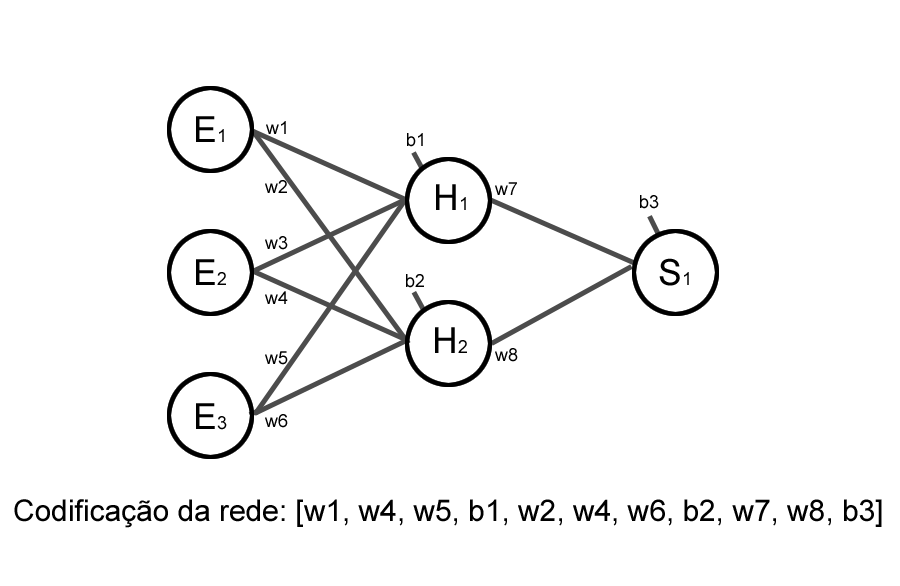
\includegraphics[width=80mm]{codificacao.png}
\caption{Codificacão da rede}
\end{figure}

\par O número de neurônios de cada camada foi especificado na tabela a seguir:


\begin{tabular}{|c|c|c|c|c|}
\hline Base  & Atributos (Entradas) & Classes (Saídas) & Escondidos \\ 
\hline Cancer & 9 & 2 & 5 \\ 
\hline Pima Indians Diabetes & 8 & 2 & 10 \\ 
\hline Glass Identification & 9 & 7 & 10 \\ 
\hline Heart & 13 & 2 & 5 \\ 
\hline Iris & 4 & 3 & 10 \\ 
\hline 
\end{tabular} 

\par O algoritmo genético foi implementado conforme \cite{essentials}. O fitness de cada indivíduo é dado pelo Erro Quadrado Médio (EQM), logo um indivíduo mais apto é aquele que possui o menor valor. O EQM é calculado de acordo com \cite{Liu}.


\par Os operadores genéticos utilizados foram:
\begin{enumerate}

	\item Operadores de Mutação, segundo \cite{montana} e \cite{Liu}:
	\begin{enumerate}
		\item Biased Mutate Weights: O valor de um gene pode ser substituído por um outro qualquer da distribuição de probabilidade inicial (distribuição normal com média 0 e desvio padrão 5).
		\item Unbiased Mutate Weights: Um valor da distribuição de probabilidade inicial é acrescido a um gene.
		\item Mutate Nodes: Este operador seleciona n neurônios das camadas oculta e de saída e adiciona um valor da distribuição de probabilidade inicial a cada peso de entrada dos neurônios. Nos nossos o valor de n foi 2.
		\item Mutate Weakest Nodes: Este operador seleciona o neurônio mais fraco (aquele que menos contribui para o saída da rede) e aplica uma mutação unbiased ou biased cada peso do neurônio mais fraco.
		\item SinglePointRandom: Cada gene do cromososmo é substituído por um valor aleatório entre [-50,50].
		\item NonUniform: implementado conforme \cite{Michalewicz}. Na nossa implementacão o parâmetro b é 4.
		
	\end{enumerate}

	\item Operadores de Crossover, segundo \cite{montana} e \cite{Liu}:
	\begin{enumerate}
		\item Crossover Weights: O valor gene de um indivíduo filho é escolhido pela seleção aleatória do mesmo gene de um dos pais.
		\item Crossover Nodes: Para cada neurônio de um dos pais escolhidos aleatoriamente o pessoas associados são passados diretamente para o filho.
		\item Crossover Features: Para cada neurônio da rede do primeiro pai, o algoritmo reorganiza o segundo pai de forma que os neurônios que desempenham o mesmo papel (isto é, possum a mesma saída para uma determinada entrada) fiquem na posição, assim formando um pai intermediário. Depois disso é aplicado o operador Crossover-Nodes entre o primeiro pai e o pai intermediário.
		\item Line Recombination: A implementação foi um hibrido entre \cite{Liu} e \cite{essentials} onde o parâmetro é dado por uma distribuição normal com média 0 e desvio padrão 5.
	\end{enumerate}

\end{enumerate}

\par Os parâmetros utilizados para o Algoritmo Genético foram os seguintes:
\begin{enumerate}
	\item Tamanho da População: 50 e 100 indivíduos;
	\item Número de Gerações: 500;
	\item Tamanho do torneio: 2 e 4;
	\item Número de indivíduos da elite: 10;
	\item Probabilidade de Crossover: 100\%;
	\item Probabilidade de mutação: 10\%.
\end{enumerate}

\par Para a análise dos resultados foi utilizado a validação cruazada \cite{Haykin:1998:NNC:521706}. Na validação cruzada o conjunto de dados é particionado aleatoriamente em um conjunto de teste e um conjunto de treinamento, que ainda é divido em um subconjunto de treinamento e um subconjunto de validação. O conjunto de dados foi separado nos seguintes grupos:


\begin{tabular}{|c|c|c|c|c|}
\hline Base & Treinamento & Validação & Teste  & Total \\ 
\hline Cancer & 350 & 175 & 174 & 699 \\ 
\hline Pima Indians Diabetes & 252 & 258 & 258 & 768 \\ 
\hline Glass Identification & 114 & 50 & 50 & 214 \\ 
\hline Heart & 130 & 70 & 70 & 270 \\ 
\hline Iris & 70 & 40 & 40 & 150 \\ 
\hline 
\end{tabular} 

















\section{Resultados obtidos}

Resultados obtidos e comparação com os resultados dos artigos estudados





\section{Considerações Finais}

Conclusões que refletem o objetivo do trabalho


\bibliographystyle{sbc}
\bibliography{sbc-template}

\end{document}
